% The Slide Definitions
%document
\documentclass[10pt]{beamer}
%theme
\usetheme{metropolis}
% packages
\usepackage{color}
\usepackage{listings}
\usepackage[ngerman]{babel}
\usepackage[utf8]{inputenc}
\usepackage{multicol}


% color definitions
\definecolor{mygreen}{rgb}{0,0.6,0}
\definecolor{mygray}{rgb}{0.5,0.5,0.5}
\definecolor{mymauve}{rgb}{0.58,0,0.82}

\lstset{
    backgroundcolor=\color{white},
    % choose the background color;
    % you must add \usepackage{color} or \usepackage{xcolor}
    basicstyle=\footnotesize\ttfamily,
    % the size of the fonts that are used for the code
    breakatwhitespace=false,
    % sets if automatic breaks should only happen at whitespace
    breaklines=true,                 % sets automatic line breaking
    captionpos=b,                    % sets the caption-position to bottom
    commentstyle=\color{mygreen},    % comment style
    % deletekeywords={...},
    % if you want to delete keywords from the given language
    extendedchars=true,
    % lets you use non-ASCII characters;
    % for 8-bits encodings only, does not work with UTF-8
    frame=single,                    % adds a frame around the code
    keepspaces=true,
    % keeps spaces in text,
    % useful for keeping indentation of code
    % (possibly needs columns=flexible)
    keywordstyle=\color{blue},       % keyword style
    % morekeywords={*,...},
    % if you want to add more keywords to the set
    numbers=left,
    % where to put the line-numbers; possible values are (none, left, right)
    numbersep=5pt,
    % how far the line-numbers are from the code
    numberstyle=\tiny\color{mygray},
    % the style that is used for the line-numbers
    rulecolor=\color{black},
    % if not set, the frame-color may be changed on line-breaks
    % within not-black text (e.g. comments (green here))
    stepnumber=1,
    % the step between two line-numbers.
    % If it's 1, each line will be numbered
    stringstyle=\color{mymauve},     % string literal style
    tabsize=4,                       % sets default tabsize to 4 spaces
    % show the filename of files included with \lstinputlisting;
    % also try caption instead of title
    language = Python,
	showspaces = false,
	showtabs = false,
	showstringspaces = false,
	escapechar = ,
}

\def\ContinueLineNumber{\lstset{firstnumber=last}}
\def\StartLineAt#1{\lstset{firstnumber=#1}}
\let\numberLineAt\StartLineAt



\newcommand{\codeline}[1]{
	\alert{\texttt{#1}}
}


% Author and Course information
% This Document contains the information about this course.

% Authors of the slides
\author{Claas de Boer, Tilman Hinnerichs}

% Name of the Course
\institute{Python-Grundlagen}

% Fancy Logo 
\titlegraphic{\hfill
\includegraphics[height=1.25cm]{../images/fsr_logo_cropped}}

% Custom Bindings
% \newcommand{\codeline}[1]{
%	\alert{\texttt{#1}}
%}


% Presentation title
\title{Fehler und Fehlermeldungen}
\date{\today}

\usepackage{tikz} \usetikzlibrary{arrows, positioning}

\tikzset{
  auto,
  invisible/.style={opacity=0},
  visible on/.style={alt={#1{}{invisible}}},
  alt/.code args={<#1>#2#3}{%
    \alt<#1>{\pgfkeysalso{#2}}{\pgfkeysalso{#3}} % \pgfkeysalso doesn't change the path
  },
}

\begin{document}

\maketitle

\section{Der Kurs in Kürze}
\begin{frame}{Der Kurs in Kürze}
    \begin{itemize}
        \item Datentypen: \texttt{int}, \texttt{str}, \texttt{float}, \ldots
        \item Kontrollstrukturen: \texttt{if}, \texttt{else}, \texttt{elif}
        \item Container: \texttt{list}, \texttt{set}, \texttt{tuple}
        \item Mapping: \texttt{dict}
        \item Objektorientierung: \texttt{class}, \texttt{init}
        \item Funktionen: \texttt{def f(x)}, \texttt{lambda f: \ldots}
        \item Built-Ins: \texttt{map}, \texttt{filter}, \texttt{zip}
        \item Dateien: \texttt{open}, \texttt{close}, \texttt{with open(\ldots) as f}
    \end{itemize}
\end{frame}

\section{Heute: Fehler \& Fehlermeldungen}

\begin{frame}[fragile]{Softwarefehler: Arianne 5}
Fehler sind menschlich, warum sollte mein Programm keine haben?
\pause
\begin{center}
    \begin{tabular}{ll}
         \begin{tabular}{l}
           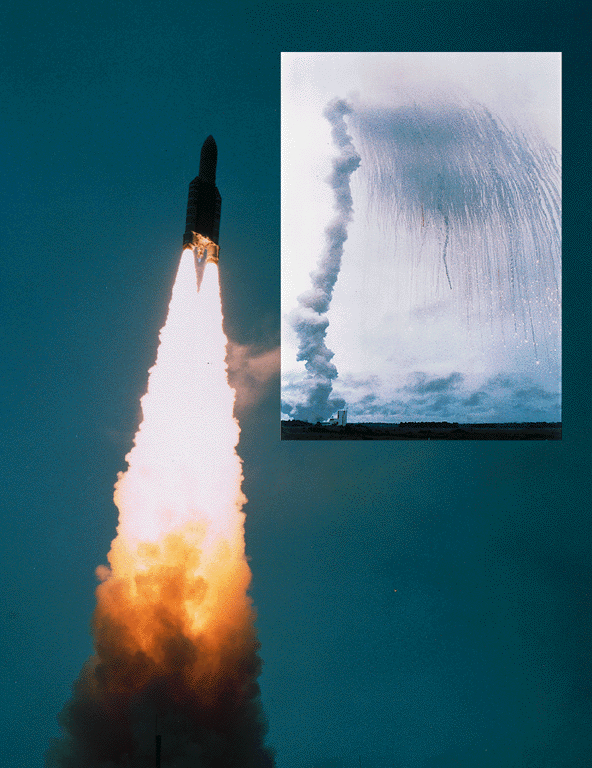
\includegraphics[height=5.5cm, width=4cm]{arianne.jpg}
           \end{tabular}
           & \begin{tabular}{l}
             \parbox{0.6\linewidth}{
                 \begin{itemize}
                     \item Erster Flug der \textbf{Arianne 5}
                     \item 4 Satteliten an Bord
                     \item Nachfolgerakete der Arianne 4
                     \item \textbf{RUD} nach 37 Sekunden
                     \item 16-Bit signed Integer Overflow (g-Sensor)
                 \end{itemize}}
        \end{tabular}\\
    \end{tabular}
\end{center}
\vspace{1em}
    \href{https://www.youtube.com/watch?v=6oXtGMBS2ho}{\textbf{Talk: Softwarefehler in der Raumfahrt}}
\end{frame}

\begin{frame}[fragile]{Softwarefehler: Python}
    Wenn Python bei der Ausführung eures Programmes einen Fehler feststellt, wird ein \textbf{Stack Trace} ausgegeben und das Programm abgebrochen.
    \pause

    Der \textbf{Stack Trace}
    \begin{itemize}
        \item enthält alle Funktionsaufrufe, die getätigt wurden bevor der Fehler auftrat,
        \item endet mit der eigentlichen Fehlermeldung
    \end{itemize}
\end{frame}

\begin{frame}[fragile]{Beispiel: NameError}
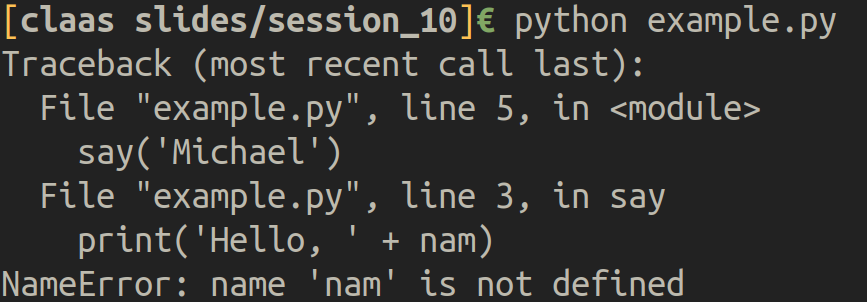
\includegraphics[width=\textwidth]{stack_trace_example.png}
\begin{lstlisting}
# example.py
def say(name):
    print('Hello, ' + nam)

say('Michael')
\end{lstlisting}
\end{frame}

\begin{frame}[fragile]{Wie liest man einen Stack Trace?}
\begin{center}
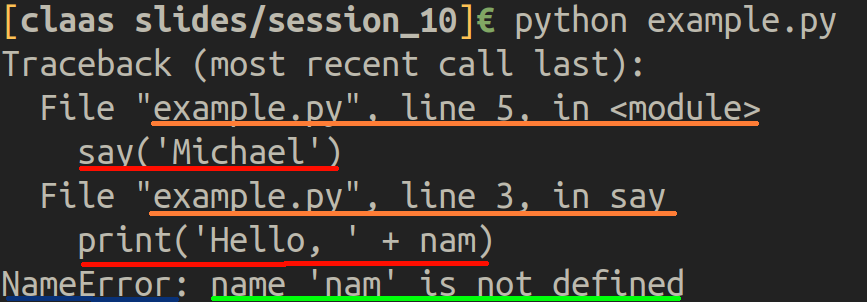
\includegraphics[width=.9\textwidth]{stack_trace_example_colored.png}
\end{center}
\begin{itemize}
    \item \textbf{Blau}: Der ausgelöste Fehler, letzte Zeile des Stack Traces
    \item \textbf{Grün}: Die Fehlernachricht (Error Message)
    \item \textbf{Orange}: Die Datei, die Zeile, und der Modulname bzw. die Funktion in welcher der Fehler aufgetreten ist
    \item \textbf{Rot}: Der ausgeführte Code, der den Fehler verursachte
\end{itemize}
\end{frame}

\section{Die beliebtesten Stack Traces: Nummer 3 wird dich überraschen!}

\begin{frame}[fragile]{Beispiel: AttributeError}
\begin{center}
    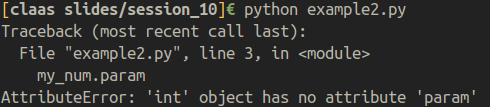
\includegraphics[width=\textwidth]{stack_trace_attribute_error.png}
\end{center}
\begin{lstlisting}
# example2.py
my_num = 1
my_num.param
\end{lstlisting}
\end{frame}

\begin{frame}[fragile]{Beispiel: ImportError}
\begin{center}
    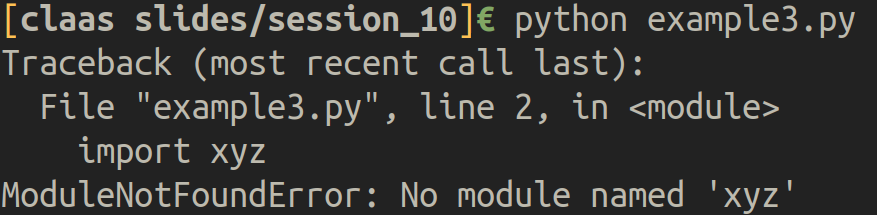
\includegraphics[width=\textwidth]{stack_trace_import_error.png}
\end{center}
\begin{lstlisting}
# example3.py
import xyz
\end{lstlisting}
\end{frame}

\begin{frame}[fragile]{Beispiel: SyntaxError}
\begin{center}
    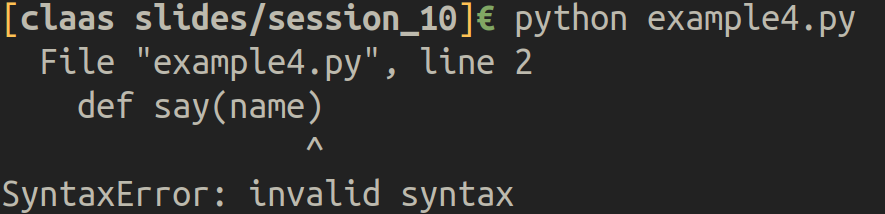
\includegraphics[width=\textwidth]{stack_trace_syntax_error.png}
\end{center}

\begin{lstlisting}
# example4.py
def say(name)
    print('Hello, ' + name)

say('Michael')
\end{lstlisting}
\end{frame}

\begin{frame}[fragile]{Beispiel: KeyError}
\begin{center}
    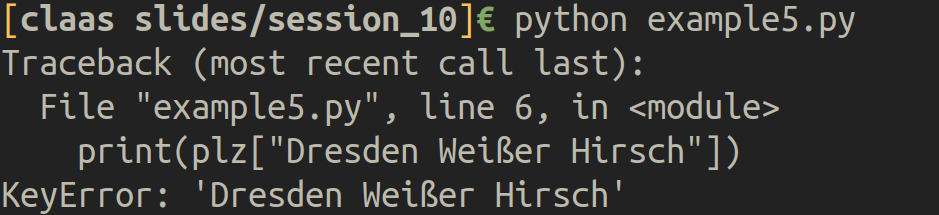
\includegraphics[width=\textwidth]{stack_trace_key_error.png}
\end{center}

\begin{lstlisting}
# example5.py
plz = {
    "Dresden Alberstadt": "01099",
    "Dresden Plauen": "01187",
    "Dresden Südvorstadt-Ost": "01217"
}
print(plz["Dresden Weißer Hirsch"])
\end{lstlisting}
\end{frame}

\begin{frame}[fragile]{Beispiel: IndexError}
\begin{center}
    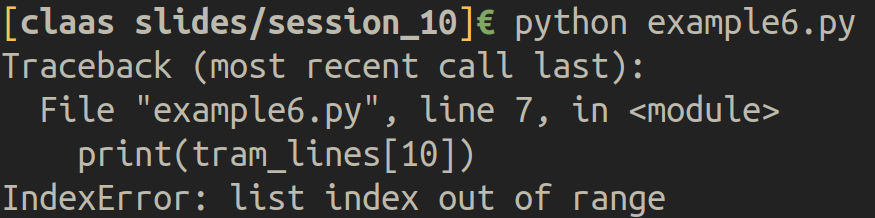
\includegraphics[width=\textwidth]{stack_trace_index_error.png}
\end{center}

\begin{lstlisting}
# example6.py
tram_lines = [
    "(7) Weixdorf - Betr. Hof Trachenberge",
    "(12) A.-Wolf-Platz - Leutewitz",
    "(46) Dresden-Niedersedlitz - Betr. Hof Trachenberge"
]
print(tram_lines[10])
\end{lstlisting}
\end{frame}

\begin{frame}[fragile]{Weitere Fehlermeldungen}
    \begin{itemize}
        \item \textbf{TypeError}: Operation an ungeeignetem Typ (Bsp: \texttt{len(13)})
        \item \textbf{ValueError}: Operation bekommt richtigen Typ, aber falschen Wert
        \item \textbf{KeyError}: Key nicht im Mapping (\texttt{dict}) vorhanden
        \item \textbf{IndexError}: Sequenzzugriff auf Element außerhalb des vorhandenen Index
        \item \textbf{IOError}: I/O Operation schlägt fehl (Bsp: Dateien)
        \item \textbf{ZeroDivisionError}: Division durch Null
        \item \ldots
    \end{itemize}
\end{frame}

\section{Fehler abfangen}

\begin{frame}[fragile]{Try, Try, and Try Again}
    Mit dem \texttt{try/except}-Statement können Fehler behandelt werden.
\begin{lstlisting}
# example2.py
my_num = 1
my_num.param
\end{lstlisting}
\begin{lstlisting}
try:
    my_num = 1
    my_num.param
except AttributeError:
    # falls im try-block ein AttributError auftritt,
    # do this
    print("Error: Property does not exist")
\end{lstlisting}
\end{frame}

\begin{frame}[fragile]{Try, Try, and Try Again - Again}
    \texttt{try/except} kann als \textbf{Catch-All} verwendet werden.
\begin{lstlisting}
try:
    func()
except Exception as e:
    print("An error occured!")
    print(e)
\end{lstlisting}
Oder um spezifische Fehler zu behandeln.
\begin{lstlisting}
try:
    func()
except ZeroDivisionError as zde:
    # handle zde
except ValueError as ve:
    # handle ve
except KeyError, IndexError as e:
    # handle KeyError & IndexError
\end{lstlisting}
\end{frame}

\begin{frame}[fragile]{Raise Exceptions from their Grave!}
    Vergleichbar mit \textbf{Built-Ins}, könnt ihr auf eine große Menge an Exceptions direkt zugreifen.

    Eine Exception auslösen könnt ihr mit dem \texttt{raise}-Statement.
\begin{lstlisting}
def series(x):
    if x < 0:
        raise ValueError
    return compute_series_for(x)
\end{lstlisting}
\end{frame}


\begin{frame}[fragile]{Aufgaben}
    \begin{enumerate}
        \item Implementiere eine Funktion \texttt{caesar\_cipher}, die für einen String \texttt{plaintext} und eine Zahl \texttt{n} den um \texttt{n} caesar-verschlüsselten String \texttt{secret} berechnet.
        \item Erweitere die Funktion \texttt{caesar\_cipher} so, dass ein TypeError ausgelöst wird, wenn die Funktion mit einem Parameter des falschen Typs aufgerufen wird. Passe die Error Message an, sodass klar wird, welcher der Parameter den Fehler ausgelöst hat.
        \item \textbf{Bonus}: Implementiere die Funktion \texttt{vigenere\_cipher}, welche die Vigenère-Chiffre implementiert.
    \end{enumerate}
\end{frame}

\begin{frame}[standout]
\begin{center}
    Vielen Dank, dass ihr so zahlreich erschienen seid!

    Habt eine schöne vorlesungsfreie Zeit.
\end{center}
\end{frame}

\end{document}
